% Math_CS_122A_HW9_Zih-Yu_Hsieh.tex

\documentclass{article}
\usepackage{graphicx} % Required for inserting images
\usepackage[margin = 2.54cm]{geometry}
\usepackage[most]{tcolorbox}

\newtcolorbox{myBox}[3]{
arc=5mm,
lower separated=false,
fonttitle=\bfseries,
%colbacktitle=green!10,
%coltitle=green!50!black,
enhanced,
attach boxed title to top left={xshift=0.5cm,
        yshift=-2mm},
colframe=blue!50!black,
colback=blue!10
}

\usepackage{amsmath}
\usepackage{amssymb}
\usepackage{verbatim}
\usepackage[utf8]{inputenc}
\linespread{1.2}

\newtheorem{definition}{Definition}
\newtheorem{proposition}{Proposition}
\newtheorem{theorem}{Theorem}
\newtheorem{question}{Question}

\title{Math CS 122A HW9}
\author{Zih-Yu Hsieh}

\begin{document}
\maketitle

\section*{1} 
\begin{myBox}[]{}
    \begin{question}
        Ahlfors Pg. 154 Problem 2:

        Hwo many roots of the equation $z^4-6z+3=0$ have their modulus between $1$ and $2$?
    \end{question}
\end{myBox}

\textbf{Pf:}

For the disk $|z|<1$, consider the function $-6z+3$: It has one zero in $|z|<1$, namely $z=\frac{1}{2}$.

On the other hand, for circle $|z|=1$, the following inequalities are true:
$$|(z^2-6z+3)-(-6z+3)| = |z|^4 = 1$$ 
$$|-6z+3| \geq |6|z|-3| = 6-3 = 3$$
So, since $|(z^2-6z+3)-(-6z+3)|=1 \leq3\leq |-6z+3|$ for all $z$ on $|z|=1$, then by Rouche's Theorem,
the two polynomials have the same number of zeroes enclosed by the circle $|z|=1$.

Since $-6z+3$ only has one zero in this region, then $z^4-6z+3$ also has one zero in this region.

\hfil

Now, consider the disk $|z|<2$, and the function $z^4$: It has four zeros in $|z|<2$ counting multiplicity (namely $z=0$).

On the other hand, for circle $|z|=2$, the following inequalities are true:
$$|(z^2-6z+3)-z^4| = |-6z+3| \leq 6|z|+3 = 15$$
$$|z^4| = |z|^4 = 16$$
So, since $|(z^4-6z+3)-z^4| = 15<16=|z^4|$ for all $z$ on $|z|=2$, by Rouche's Theorem again, the two polynomials have the same number of zeroes enclosed by the circle $|z|=2$.
Since $z^4$ has four zeroes in this region, then $z^4-6z+3$ also has four zeroes in this region.

\hfil

Then, since $4$ zeroes has modulus less than $2$, while $1$ zero has modulus less than $1$, counting the ones with modulus between $1$ and $2$,
we have total of $4-1=3$ zeroes.

\break

\section*{2}
\begin{myBox}[]{}
    \begin{question}
        Ahlfors Pg. 161 Problem 5:

        Complex integration can sometimes be used to evaluate area integrals. 
        As an illustration, show that if $f(z)$ is analytic and bounded for $|z|<1$ and if $|\zeta|<1$, then
        $$f(\zeta)=\frac{1}{\pi}\int\int_{|z|<1}\frac{f(z)dxdy}{(1-\bar{z}\zeta)^2}$$
    \end{question}
\end{myBox}

\textbf{Pf:}

If convert the above integral to polar coordinates, we get the following:
$$\frac{1}{\pi}\int\int_{|z|<1}\frac{f(z)dxdy}{(1-\bar{z}\zeta)^2}=\frac{1}{\pi}\int_{r=0}^{1}\int_{\theta=0}^{2\pi}\frac{f(re^{i\theta})r}{(1-\zeta re^{-i\theta})^2}d\theta dr = \frac{1}{\pi}\int_{r=0}^{1}\int_{\theta=0}^{2\pi}\frac{f(re^{i\theta})(e^{i\theta})^2\cdot r}{(e^{i\theta}-r\zeta)^2}d\theta dr$$
Then, define $C$ to have parametrization $z=e^{i\theta}$ with $\theta\in [0,\pi]$, the inner part of the integral becomes:
$$\frac{1}{\pi}\int_{\theta=0}^{2\pi}\frac{f(re^{i\theta})(e^{i\theta})^2r}{(e^{i\theta}-r\zeta)^2}d\theta =2\cdot \frac{1}{2\pi i}\int_{0}^{\pi}\frac{f(re^{i\theta})re^{i\theta}}{(e^{i\theta}-r\zeta)^2}ie^{i\theta}d\theta = 2\cdot\frac{1}{2\pi i}\int_{C}\frac{f(rz)rz}{(z-r\zeta)^2}dz$$
Recall that for any analytic function $\phi(z)$ at a point $a$, by Cauchy's Integral formula, we get:
$$\phi'(a)=\frac{1!}{2\pi i}\int_{C}\frac{\phi(z)}{(z-a)^2}dz$$
So, given that $z=r\zeta$ (which with $r\in [0,1]$ and $|\zeta|<1$, $r\zeta$ is strictly in the unit disk, so integrate over $C$ given above is valid), let $\phi(z)=f(rz)rz$ (which $\phi'(z)=f'(rz)r^2z + f(rz)r$), we have:
$$f'(r(r\zeta))r^2(r\zeta) + f(r(r\zeta))r = \frac{1!}{2\pi i}\int_{C}\frac{f(rz)rz}{(z-r\zeta)^2}dz$$
$$2\cdot\frac{1}{2\pi i}\int_{C}\frac{f(rz)rz}{(z-r\zeta)^2}dz = 2\left(f'(r^2\zeta)r^3\zeta + f(r^2\zeta)r\right)$$
Hence, the original integral can be rewrite as:
$$\frac{1}{\pi}\int_{r=0}^{1}\int_{\theta=0}^{2\pi}\frac{f(re^{i\theta})(e^{i\theta})^2\cdot r}{(e^{i\theta}-r\zeta)^2}d\theta dr = \int_{r=0}^{1}2\left(f'(r^2\zeta)r^3\zeta + f(r^2\zeta)r\right) dr$$
Now, consider the function $f(\zeta r^2)r^2$, which has derivative $f'(\zeta r^2)r^2\cdot 2r\zeta + f(\zeta r^2)\cdot 2r = 2\left(f'(r^2\zeta)r^3\zeta + f(r^2\zeta)r\right)$. 
Then, the above integral can be rewrite as:
$$\int_{r=0}^{1}2\left(f'(r^2\zeta)r^3\zeta + f(r^2\zeta)r\right) dr = f(\zeta r^2)r^2\bigg|_{r=0}^{1} = f(\zeta)$$
Hence, we can claim that for $f(z)$ that's analytic and bounded on $|z|<1$, and given $|\zeta|<1$, the integral is true:
$$f(\zeta)=\frac{1}{\pi}\int\int_{|z|<1}\frac{f(z)dxdy}{(1-\bar{z}\zeta)^2}$$

\break

\section*{3}
\begin{myBox}[]{}
    \begin{question}
        Stein and Shakarchi Pg. 64 Problem 1:

        Prove that
        $$\int_{0}^{\infty}\sin(x^2)dx = \int_{0}^{\infty}\cos(x^2)dx = \frac{\sqrt{2\pi}}{4}$$
    \end{question}
\end{myBox}

\textbf{Pf:}

Consider the function $e^{-z^2}$, and the integration over a sector with origin at $0$ and radius $R$.
Which, this can be parametrized by three curves: $\gamma_1$ - a straight line on real axis with $x\in[0,R]$, 
$\gamma_2$ - a circular arc with radian $\frac{\pi}{4}$ and radius $R$ (parametrized by $z=Re^{i\theta}$, where $\theta\in [0,\frac{\pi}{4}]$),
and $\gamma_3$ - another straight line of $z=re^{i\frac{\pi}{4}}$ (where $r\in [0,R]$). The orientation is given as follow:

\begin{center}
    \includegraphics*[width=60mm]{problem 3.png}
\end{center}

If consider the integral over this closed curve, since $e^{-z^2}$ is analytic on the whole plane, then the line integral is $0$. So, $\int_{\gamma_1+\gamma_2+\gamma_3}e^{-z^2}dz=0$.

\hfil

For $\int_{\gamma_1}e^{-z^2}dz$, it is parametrized by $\int_{0}^{R}e^{-x^2}dx$, which $\lim_{R\rightarrow\infty}\int_{0}^{R}e^{-x^2}dx=\frac{\sqrt{\pi}}{2}$ (since $e^{-x^2}$ is even, while $\int_{-\infty}^{\infty}e^{-x^2}dx=\sqrt{\pi}$).

\hfil

For $\int_{\gamma_2}e^{-z^2}dz$, it is parametrized by the following:
$$\int_{\gamma_2}e^{-z^2}dz=\int_{0}^{\frac{\pi}{4}}\exp\left(-(Re^{i\theta})^2\right)iRe^{i\theta}d\theta = \int_{0}^{\frac{\pi}{4}}\exp(-R^2e^{i2\theta})iRe^{i\theta}d\theta$$
$$= \int_{0}^{\frac{\pi}{4}}\exp(-R^2(\cos(2\theta)+i\sin(2\theta)))iRe^{i\theta}d\theta = \int_{0}^{\frac{\pi}{4}}e^{-R^2\cos(2\theta)}e^{-iR^2\sin(2\theta)}iRe^{i\theta}d\theta$$
Which, consider the modulus, the following inequality is true:
$$\left|\int_{\gamma_2}e^{-z^2}dz\right|\leq \int_{0}^{\frac{\pi}{4}}|e^{-R^2\cos(2\theta)}|\cdot |e^{-iR^2\sin(2\theta)}|\cdot |iRe^{i\theta}|d\theta = \int_{0}^{\frac{\pi}{4}}Re^{-R^2\cos(2\theta)}d\theta$$
$$\left|\int_{\gamma_2}e^{-z^2}dz\right|\leq \frac{1}{2}\int_{0}^{\frac{\pi}{2}}Re^{-R^2\cos(u)}du$$
(Note: the second line is done by the parametrization $u=2\theta$).

Now, since in the domain $[0,\frac{\pi}{2}]$, $1-\frac{2}{\pi}u \leq \cos(u)$, then $e^{-R^2\cos(u)}\leq e^{-R^2(1-\frac{2}{\pi}u)}$ (given that $-R^2<0$, while the two functions are positive on the given domain).
Then, we can further bound the integral by:
$$\left|\int_{\gamma_2}e^{-z^2}dz\right|\leq \frac{1}{2}\int_{0}^{\frac{\pi}{2}}Re^{-R^2\cos(u)}du \leq \frac{1}{2}\int_{0}^{\frac{\pi}{2}}Re^{-R^2(1-\frac{2}{\pi}u)}du=\frac{1}{2}\int_{0}^{\frac{\pi}{2}}Re^{R^2\cdot\frac{2}{\pi}u-R^2}du$$
$$\leq \frac{R}{2}\cdot\frac{\pi}{2R^2}e^{R^2\cdot \frac{2}{\pi}u-R^2}\bigg|_{0}^{\frac{\pi}{2}} = \frac{\pi}{4R}(e^{R^2\cdot\frac{2}{\pi}\cdot\frac{\pi}{2}-R^2}-e^{R^2\cdot\frac{2}{\pi}\cdot 0-R^2}) = \frac{\pi}{4R}(1-e^{-R^2})$$
Then, since $\lim_{R\rightarrow\infty}\frac{\pi}{4R}=0$, $\lim_{R\rightarrow\infty}(1-e^{-R^2})=1$, then:
$$0\leq \lim_{R\rightarrow\infty}\left|\int_{\gamma_2}e^{-z^2}dz\right|\leq \lim_{R\rightarrow\infty} \frac{\pi}{4R}(1-e^{-R^2})=0$$
Hence, we can claim that $\lim_{R\rightarrow\infty}\int_{\gamma_2}e^{-z^2}dz = 0$.

\hfil

Lastly, for $\int_{\gamma_3}e^{-z^2}dz$, it is parametrized by $\int_{R}^{0}\exp(-(re^{i\frac{\pi}{4}})^2)e^{i\frac{\pi}{4}}dr$. Which, can be modified as:
$$\int_{R}^{0}\exp(-r^2e^{i\frac{\pi}{2}})e^{i\frac{\pi}{4}}dr = e^{i\frac{\pi}{4}}\int_{R}^{0}e^{-ir^2}dr = e^{i\frac{\pi}{4}}\left(\int_{R}^{0}\cos(r^2)dr - i\int_{R}^{0}\sin(r^2)dr\right)$$
$$=-e^{i\frac{\pi}{4}}\left(\int_{0}^{R}\cos(r^2)dr - i\int_{0}^{R}\sin(r^2)dr\right)$$

Now, because $\int_{\gamma_1+\gamma_2+\gamma_3}e^{-z^2}dz=0$, then $\int_{\gamma_3}e^{-z^2}dz = -(\int_{\gamma_1}e^{-z^2}dz+\int_{\gamma_2}e^{-z^2}dz)$. Hence:
$$\lim_{R\rightarrow\infty}\int_{\gamma_3}e^{-z^2}dz = \lim_{R\rightarrow\infty}-\left(\int_{\gamma_1}e^{-z^2}dz+\int_{\gamma_2}e^{-z^2}dz\right) = -\frac{\sqrt{\pi}}{2}$$
$$\lim_{R\rightarrow\infty}-e^{i\frac{\pi}{4}}\left(\int_{0}^{R}\cos(r^2)dr - i\int_{0}^{R}\sin(r^2)dr\right) = -\frac{\sqrt{\pi}}{2}$$
Hence, we can claim the following:
$$\int_{0}^{\infty}\cos(r^2)dr - i\int_{0}^{\infty}\sin(r^2)dr = \frac{\sqrt{\pi}}{2}e^{-i\frac{\pi}{4}} = \frac{\sqrt{2\pi}}{4}(1-i)$$
Then, take the real and imaginary part respectively, we get:
$$\int_{0}^{\infty}\cos(r^2)dr = Re\left(\frac{\sqrt{2\pi}}{4}(1-i)\right)=\frac{\sqrt{2\pi}}{4}$$
$$\int_{0}^{\infty}\sin(r^2)dr = -Im\left(\frac{\sqrt{2\pi}}{4}(1-i)\right)=\frac{\sqrt{2\pi}}{4}$$
Hence, the two integrals evaluated to be $\frac{\sqrt{2\pi}}{4}$.

\break

\section*{4}
\begin{myBox}[]{}
    \begin{question}
        Stein and Shakarchi Pg. 65 Problem 4:

        Prove that for all $\zeta\in \mathbb{C}$ we have 
        $$e^{-\pi \zeta^2}=\int_{-\infty}^{\infty}e^{-\pi x^2}e^{2\pi ix\zeta}dx$$
    \end{question}
\end{myBox}

\textbf{Pf:}

Given $\zeta=u+iv$ for some $u,v\in\mathbb{R}$. Consider the function $e^{-\pi z^2}$ which is analytic on $\mathbb{C}$.
There are three cases:
\begin{itemize}
    \item[(1)] \textbf{When $u>0$}, given $R>0$, consider the parallelagram generated by the points $-R,R,R+i\zeta,-R+i\zeta$ with counterclockwise orientation. The orientation is as follow:
    
    \begin{center}
        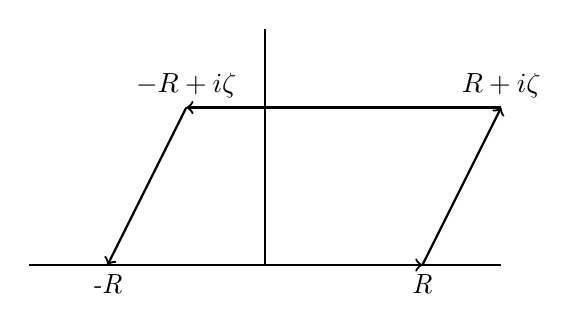
\begin{tikzpicture}
            % Define points
            \coordinate (A) at (-2,0);
            \coordinate (B) at (2,0);
            \coordinate (C) at (3,2);
            \coordinate (D) at (-1,2);
            \coordinate (Mid) at (0,0);
            \coordinate (TopMid) at (1,2);
            
            % Draw base line
            \draw[thick] (A) -- (B);
            
            % Draw vertical middle line
            \draw[thick] (-3,0) -- (3,0);
            \draw[thick] (0,0) -- (0,3);
            
            % Draw inclined lines
            \draw[thick,->] (B) -- (C);
            \draw[thick,->] (C) -- (D);
            \draw[thick,->] (D) -- (A);
            
            % Draw current direction on base
            \draw[thick,->] (Mid) -- (B);
            
            % Label resistance values
            \node[below] at (A) {\textit{-R}};
            \node[below] at (B) {\textit{R}};
            
            % Label points on the top
            \node[above] at (D) {\textit{$-R + i\zeta$}};
            \node[above] at (C) {\textit{$R + i\zeta$}};
        \end{tikzpicture}
    \end{center}

    Then, the integral of $e^{-\pi z^2}$ on the contour is $0$ (since it is analytic on the whole plane). Which, it can be broken down into the sum of following integrals:

    \hfil

    First, for the one on the real axis, it is parametrized by $\int_{-R}^{R}e^{-\pi x^2}dx$, where $\lim_{R\rightarrow\infty}\int_{-R}^{R}e^{-\pi x^2}dx=1$ (Gauss Integral).

    \hfil

    For the ones on the side, since the sides are parametrized by $R+i\zeta t$ and $-R+i\zeta t$ for $t\in[0,1]$ respectively, then the first integral is given by:
    $$\int_{0}^{1}e^{-\pi(R+i\zeta t)^2}\cdot i\zeta dt = \int_{0}^{1}e^{-\pi(R^2+i\cdot 2R\zeta t-\zeta^2t^2)}\cdot i\zeta dt$$
    $$=\int_{0}^{1}e^{-\pi(R^2-2Rvt)}\cdot e^{-i\cdot 2\pi Rut+\pi\zeta^2t^2}\cdot i\zeta dt=e^{-\pi R^2}\int_{0}^{1}e^{R\cdot 2\pi vt}\cdot e^{-i\cdot 2\pi Rut}\cdot e^{\pi\zeta^2t^2}\cdot i\zeta dt$$
    Which, taking the modulus, it is bounded by:
    $$\left|\int_{0}^{1}e^{-\pi(R+i\zeta t)^2}\cdot i\zeta dt\right| \leq e^{-\pi R^2}\int_{0}^{1}e^{R\cdot 2\pi vt}\cdot |e^{-i\cdot 2\pi Rut}|\cdot |e^{\pi\zeta^2t^2}|\cdot |i\zeta| dt$$
    $$\leq e^{-\pi R^2}\int_{0}^{1}e^{R\cdot |2\pi v|}\cdot |e^{\pi\zeta^2t^2}|\cdot |\zeta| dt = e^{\pi R^2+R\cdot |2\pi v|}\int_{0}^{1}\cdot |e^{-\pi \zeta^2t^2}|\cdot |\zeta| dt$$
    (Note: the above is given by $R\cdot 2\pi vt \leq R\cdot |2\pi v|\cdot t \leq R\cdot|2\pi v|$, since $t\in [0,1]$).

    Then, since $\lim_{R\rightarrow\infty}-\pi R^2+R|2\pi v| = -\infty$, so $\lim_{R\rightarrow\infty}e^{-\pi R^2+R|2\pi v|}=0$, then since $\int_{0}^{1}\cdot |e^{\pi\zeta^2t^2}|\cdot |\zeta| dt$ is a constant, then:
    $$\lim_{R\rightarrow\infty}e^{-\pi R^2+R\cdot |2\pi v|}\int_{0}^{1}\cdot |e^{-\zeta^2t^2}|\cdot |\zeta| dt = 0$$
    So, we can conclude the following:
    $$\lim_{R\rightarrow\infty}\int_{0}^{1}e^{-\pi(R+i\zeta t)^2}\cdot i\zeta dt = 0$$

    Similar concepts applied on the line $-R+i\zeta t$ (since $-\pi(-R+i\zeta t)^2$ is then given by $-\pi(R^2+2Rvt)-\pi(-i\cdot 2Rut-\zeta^2t^2)$, so the same concept still applies, where the bound of the modulus is dominated by $e^{-\pi(R^2+2Rv)}$, 
    which converges to $0$ as $R\rightarrow\infty$). Hence: 
    $$\lim_{R\rightarrow\infty}\int_{0}^{1}e^{-\pi(-R+i\zeta t)^2}\cdot i\zeta dt = 0$$

    \hfil

    Lastly, the translated line is parametrized by $x+i\zeta$ for $x\in [-R,R]$, then the integral is given by:
    $$\int_{-R}^{R}e^{-\pi(x+i\zeta)^2}dx = \int_{-R}^{R}e^{-\pi(x^2+2ix\zeta - \zeta^2)}dx = e^{\pi\zeta^2}\int_{-R}^{R}e^{-\pi x^2}\cdot e^{-2\pi ix\zeta}dx$$
    
    \hfil

    Now, summing up all the path integrals with right orientation, we get the following:
    $$\int_{-R}^{R}e^{-\pi x^2}dx+\int_{0}^{1}e^{-\pi(R+i\zeta t)^2}\cdot i\zeta dt -\int_{0}^{1}e^{-\pi(-R+i\zeta t)^2}\cdot i\zeta dt-\int_{-R}^{R}e^{-\pi(x+i\zeta)^2}dx=0$$
    $$\int_{-R}^{R}e^{-\pi(x+i\zeta)^2}dx=\int_{-R}^{R}e^{-\pi x^2}dx+\int_{0}^{1}e^{-\pi(R+i\zeta t)^2}\cdot i\zeta dt -\int_{0}^{1}e^{-\pi(-R+i\zeta t)^2}\cdot i\zeta dt$$
    So, take $R\rightarrow\infty$, the first term on the right approaches $1$, while the next two terms converges to $0$ (from the above statements), then the limit becomes:
    $$\lim_{R\rightarrow\infty}\int_{-R}^{R}e^{-\pi(x+i\zeta)^2}dx = \lim_{R\rightarrow\infty}e^{\pi\zeta^2}\int_{-R}^{R}e^{-\pi x^2}\cdot e^{-2\pi ix\zeta}dx = 1$$
    So, we can conclude that $\int_{-\infty}^{\infty}e^{-\pi x^2}\cdot e^{-2\pi ix\zeta}dx = e^{-\pi\zeta^2}$.

    Which, by doing substitution $u=-x$ ($-du=dx$), we get the following:
    $$-\int_{\infty}^{-\infty}e^{-\pi u^2}\cdot e^{-2\pi i(-u)\zeta} du = \int_{-\infty}^{\infty}e^{-\pi u^2}\cdot e^{2\pi iu\zeta}du = e^{-\pi\zeta^2}$$

    \hfil

    \begin{comment}
    \item[(2)] \textbf{When $u<0$}, similar constructions can be made, but instead using $-R,R,R-i\zeta,-R-i\zeta$ as the four points instead.
    
    \begin{center}
        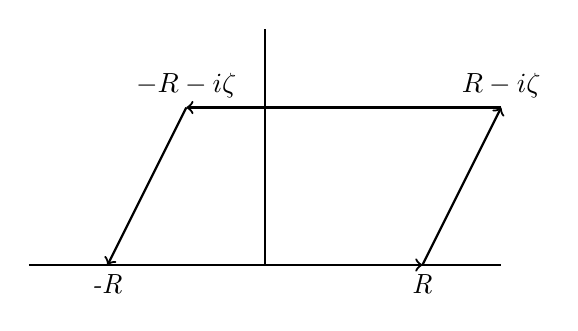
\begin{tikzpicture}
            % Define points
            \coordinate (A) at (-2,0);
            \coordinate (B) at (2,0);
            \coordinate (C) at (3,2);
            \coordinate (D) at (-1,2);
            \coordinate (Mid) at (0,0);
            \coordinate (TopMid) at (1,2);
            
            % Draw base line
            \draw[thick] (A) -- (B);
            
            % Draw vertical middle line
            \draw[thick] (-3,0) -- (3,0);
            \draw[thick] (0,0) -- (0,3);
            
            % Draw inclined lines
            \draw[thick,->] (B) -- (C);
            \draw[thick,->] (C) -- (D);
            \draw[thick,->] (D) -- (A);
            
            % Draw current direction on base
            \draw[thick,->] (Mid) -- (B);
            
            % Label resistance values
            \node[below] at (A) {\textit{-R}};
            \node[below] at (B) {\textit{R}};
            
            % Label points on the top
            \node[above] at (D) {\textit{$-R - i\zeta$}};
            \node[above] at (C) {\textit{$R - i\zeta$}};
        \end{tikzpicture}
    \end{center}

    (Note: For this part, $i\zeta$ has imaginary part $u$, then $-i\zeta$ has imaginary part $-u$, which is positive).
    
    (Note 2: the reason using $-i$, is because we want the integration to be over a counterclockwise orientation).

    Using similar concept, we can prove the exact same result as $u>0$ (where the contour integral is $0$):

    \hfil

    For the line integral on real axis, $\lim_{R\rightarrow\infty}\int_{-R}^{R}e^{-\pi x^2}dx=1$ again based on Gauss's Integral.

    \hfil

    For side integrals parametrized by $R-i\zeta t$ and $-R-i\zeta t$ (with $t\in[0,1]$), we can expand the integrals to following form:
    $$I_1=\int_{0}^{1}e^{-\pi(R-i\zeta t)^2}\cdot (-i\zeta)dt = e^{-\pi R^2}\int_{0}^{1}e^{-R\cdot 2\pi vt}\cdot e^{i\cdot 2\pi Rut}\cdot e^{\pi\zeta^2 t^2}(-i\zeta)dt$$
    $$I_2 = \int_{0}^{1}e^{-\pi(-R-i\zeta t)^2}\cdot (-i\zeta)dt = e^{-\pi R^2}\int_{0}^{1}e^{-R\cdot 2\pi vt}\cdot e^{-i\cdot 2\pi Rut}\cdot e^{\pi\zeta^2 t^2}(-i\zeta)dt$$
    Again, using the same inequality $(e^{-R\cdot 2\pi vt} \leq e^{R|2\pi v|}$, and the fact that $\lim_{R\rightarrow\infty}e^{-\pi R^2+R|2\pi v|}=0$), we get:
    $$\lim_{R\rightarrow\infty}|I_1| \leq \lim_{R\rightarrow\infty}e^{-\pi R^2}\int_{0}^{1}e^{-R\cdot 2\pi vt}\cdot |e^{i\cdot 2\pi Rut}|\cdot |e^{\pi\zeta^2 t^2}|\cdot|-i\zeta|dt$$
    $$\leq \lim_{R\rightarrow\infty}e^{-\pi R^2+R|2\pi v|}\int_{0}^{1}|e^{\pi\zeta^2 t^2}|\cdot |\zeta|dt = 0$$
    Similar inequality applies for $|I_2|$, hence as $R\rightarrow\infty$, $I_1,I_2$ both converges to $0$ (since the modulus converges to $0$).

    \hfil

    Lastly, for the upper half of the parallelagram parametrized by $x-i\zeta$ for $\in [-R,R]$, we get:
    $$\int_{-R}^{R}e^{-\pi(x-i\zeta)^2}dx = \int_{-R}^{R}e^{-\pi (x^2-2ix\zeta)}$$
    \end{comment}
    
    \item[(2)] \textbf{When $u=0$}, since $\zeta=iv$, then $\zeta^2 = -v^2$. So, the proposed integral becomes:
    $$\int_{-R}^{R}e^{-\pi x^2}\cdot e^{2\pi ix\zeta}dx = \int_{-R}^{R}e^{-\pi x^2}\cdot e^{2\pi ix\cdot iv}dx = \int_{-R}^{R}e^{-\pi x^2}\cdot e^{-2\pi vx}dx$$
    Which, by completing the square, we get:
    $$\int_{-R}^{R}e^{-\pi x^2}\cdot e^{2\pi ix\zeta}dx = e^{\pi v^2}\int_{-R}^{R}e^{-\pi x^2}\cdot e^{-2\pi vx}\cdot e^{-\pi v^2}dx = e^{\pi v^2}\int_{-R}^{R}e^{-\pi(x^2+2vx+v^2)}dx = e^{\pi v^2}\int_{-R}^{R}e^{-\pi(x+v)^2}dx$$
    Then, as $R\rightarrow\infty$, we get:
    $$\lim_{R\rightarrow\infty}\int_{-R}^{R}e^{-\pi x^2}\cdot e^{2\pi ix\zeta}dx=\lim_{R\rightarrow\infty}e^{\pi v^2}\int_{-R}^{R}e^{-\pi(x+v)^2}dx = e^{\pi v^2}\int_{-\infty}^{\infty}e^{-\pi(x+v)^2}dx = e^{\pi v^2}$$
    And, since $e^{\pi v^2}=e^{-\pi \zeta^2}$, then:
    $$e^{-\pi \zeta^2} = \int_{-\infty}^{\infty}e^{-\pi x^2}\cdot e^{2\pi ix\zeta}dx$$
\end{itemize}

\hfil

So, regardless of the case, we can say that the following integral is true:
$$e^{-\pi \zeta^2} = \int_{-\infty}^{\infty}e^{-\pi x^2}\cdot e^{2\pi ix\zeta}dx$$

\hfil

\hfil

\section*{5}
\begin{myBox}[]{}
    \begin{question}
        Stein and Shakarchi Pg. 103 Problem 5:

        Use contour integration to show that for all $\zeta$ real
        $$\int_{-\infty}^{\infty}\frac{e^{-2\pi ix\zeta}}{(1+x^2)^2}dx = \frac{\pi}{2}(1+2\pi |\zeta|)e^{-2\pi |\zeta|}$$
    \end{question}
\end{myBox}

\textbf{Pf:}

\textbf{Residue at $i,-i$:}

Consider the function $f(z)=e^{-2\pi i\zeta z}/(1+z^2)^2 = e^{-2\pi i\zeta z}/((z-i)(z+i))^2$, which it has poles at $z=\pm i$, each with order $2$ (since $(z^2+1)^2=(z-i)^2(z+i)^2$).

Then, to show its residue at $i$, consider the derivative of $\phi_i(z)=e^{-2\pi i\zeta z}/(z+i)^2$:
$$\phi_i'(z) = \frac{-2\pi i\zeta e^{-2\pi i\zeta z}\cdot (z+i)^2-2(z+i)e^{-2\pi i\zeta z}}{(z+i)^4}, \quad\phi_i'(i)=\frac{-2\pi i\zeta e^{2\pi \zeta}(-4)-2(2i)e^{2\pi \zeta}}{16} = -\frac{1}{4}(1-2\pi \zeta)ie^{2\pi \zeta}$$
Then, we can expand $\phi_i(z)$ as the following term:
$$\phi_i(z) = \phi_i(i)+\phi_i'(i)(z-i)+\phi_{i,2}(z)(z-i)^2$$
The above term has $\phi_{i,2}(z)$ being analytic at $i$. Hence, $f(z)$ can be represented as:
$$f(z)=\frac{\phi_i(z)}{(z-i)^2}=\frac{\phi_i(i)}{(z-i)^2}+\frac{\phi_i'(i)}{(z-i)}+\phi_{i,2}(z)$$
Because the first term has antiderivative, while the third term is analytic at $i$, then for sufficiently small circle $C$ centered at $i$, the residue is given by:
$$Res_{z=i}f(z)=\frac{1}{2\pi i}\int_{C}\frac{\phi_i'(i)}{(z-i)}dz = n(C,i)\cdot \phi_i'(i) = -\frac{1}{4}(1-2\pi \zeta)ie^{2\pi \zeta}$$

\hfil

Now, apply similar concept for $z=-i$, the derivative of $\phi_{-i}(z)=e^{-2\pi i\zeta z}/(z-i)^2$ is given as:
$$\phi_{-i}'(z)=\frac{-2\pi i\zeta e^{-2\pi i\zeta z}\cdot (z-i)^2-2(z-i)e^{-2\pi i\zeta z}}{(z-i)^4},\quad \phi_{-i}'(-i)=\frac{-2\pi i\zeta e^{-2\pi\zeta}(-4)-2(-2i)e^{-2\pi\zeta}}{16}=\frac{1}{4}(1+2\pi\zeta)ie^{-2\pi\zeta}$$
Then, expand $\phi_{-i}(z)$ as follow:
$$\phi_{-i}(z)=\phi_{-i}(-i)+\phi_{-i}'(-i)(z+i)^2+\phi_{-i,2}(z)(z+i)^2$$
Then, the above term has $\phi_{-i,2}(z)$ being analytic at $i$. Hence, $f(z)$ can again be represented as:
$$f(z)=\frac{\phi_{-i}(z)}{(z+i)^2}=\frac{\phi_{-i}(-i)}{(z+i)^2}+\frac{\phi_{-i}'(-i)}{(z+i)}+\phi_{-i,2}(z)$$
Therefore, based on similar reason as above (where the first and third terms are analytic or has antiderivative), with a sufficiently small circle $C$ centered at $-i$, the residue at $-i$ is given as:
$$Res_{z=-i}f(z)=\frac{1}{2\pi i}\int_{C}\frac{\phi_{-i}'(-i)}{(z+i)}dz = n(C,-i)\phi_{-i}'(-i)=\frac{1}{4}(1+2\pi\zeta)ie^{-2\pi\zeta}$$

\hfil

\textbf{Integration for $\zeta\geq 0$:}

Choose a radius $R>1$, and consider a semicircle $C_R$ in lower half plane parametrized by $z=Re^{-i\theta}$ with $\theta\in [0,\pi]$, and another straight line with $-R\leq x\leq R$ with the following orientation:

\begin{center}
    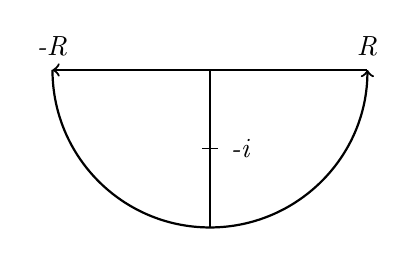
\begin{tikzpicture}
        % Draw horizontal base line
        \draw[->,thick] (2,0) -- (-2,0);
        
        % Draw vertical radius
        \draw[thick] (0,0) -- (0,-2);
        
        % Indicate current direction
        \draw[->,thick] (-2,0) arc[start angle=180,end angle=360,radius=2cm];
        
        % Small tick mark at center
        \draw (-0.1,-1) -- (0.1,-1);
        
        % Label current 'i'
        \node at (0.4,-1) {\textit{-i}};

        % label 'R' and '-R'
        \node at (2,0.3) {\textit{R}};
        \node at (-2,0.3) {\textit{-R}};
    \end{tikzpicture}
\end{center}

Since it encloses only $z=-i$, if we integrate $f(z)$ along the contour of the semicircle, we'll get:
$$\int_{R}^{-R}f(x)dx + \int_{C_R}f(z)dz = 2\pi i \cdot Res_{z=-i}f(z) = 2\pi i\cdot (\frac{1}{4}(1+2\pi\zeta)ie^{-2\pi\zeta}) = -\frac{\pi}{2}(1+2\pi\zeta)e^{-2\pi\zeta}$$
Now, consider the second integral above with the parametrization:
$$\int_{C_R}f(z)dz = \int_{\pi}^{0}\frac{e^{-2\pi i\zeta Re^{-i\theta}}}{(1+(Re^{-i\theta})^2)^2}\cdot (-iR)e^{-i\theta}d\theta$$
Since $Re^{-i\theta}=R\cos(\theta)-i\cdot R\sin(\theta)$, then the exponential part could be rewrite as:
$$e^{-2\pi i\zeta Re^{-i\theta}} = e^{-2\pi i\zeta (R\cos(\theta)-i\cdot R\sin(\theta))} = e^{-2\pi R\zeta\sin(\theta)}\cdot e^{-i\cdot 2\pi R\zeta\cos(\theta)}$$
Hence, if we take the modulus, the following inequality is true:
$$\left|\int_{C_R}f(z)dz\right| = \left|-\int_{0}^{\pi}\frac{e^{-2\pi i\zeta Re^{-i\theta}}}{(1+(Re^{-i\theta})^2)^2}\cdot (-iR)e^{-i\theta}d\theta\right|$$
$$\leq \int_{0}^{\pi}\frac{|e^{-2\pi i\zeta Re^{-i\theta}}|}{|1+(Re^{-i\theta})^2|^2}\cdot|-iRe^{-i\theta}|d\theta \leq \int_{0}^{\pi}\frac{e^{-2\pi R\zeta \sin(\theta)}}{(R^2-1)^2}R d\theta$$
Since $2\pi R\zeta\sin(\theta)\geq 0$ for $\theta\in [0,\pi]$ (since $\zeta\geq 0$ in this section), $e^{-2\pi R\zeta\sin(\theta)}\leq 1$. Then the above integral can then be bounded by:
$$\left|\int_{C_R}f(z)dz\right|\leq \int_{0}^{\pi}\frac{R}{(R^2-1)^2}d\theta = \frac{\pi R}{(R^2-1)^2}$$
So, as $R$ grows indefinitely, we get:
$$0\leq \lim_{R\rightarrow\infty}\left|\int_{C_R}f(z)dz\right|\leq \lim_{R\rightarrow\infty}\frac{\pi R}{(R^2-1)^2}=0$$
Hence, $\lim_{R\rightarrow\infty}\int_{C_R}f(z)dz=0$.

So, we can claim that $\lim_{R\rightarrow\infty}\int_{R}^{-R}f(x)dx + \int_{C_R}f(z)dz = \int_{\infty}^{-\infty}f(x)dx = -\frac{\pi}{2}(1+2\pi\zeta)e^{-2\pi\zeta}$, so $\int_{-\infty}^{\infty}f(x)dx = \frac{\pi}{2}(1+2\pi\zeta)e^{-2\pi\zeta}$.

Since $\zeta\geq 0$, then it can also be characterized as:
$$\int_{-\infty}^{\infty}f(x)dx = \int_{-\infty}^{\infty}\frac{e^{-2\pi ix\zeta}}{(1+x^2)^2}dx = \frac{\pi}{2}(1+2\pi|\zeta|)e^{-2\pi|\zeta|}$$

\hfil

\textbf{Integration for $\zeta<0$:}

Choose a radius $R>1$, and the semicircle $C_R$ in the upper half plane parametrized by $z=Re^{i\theta}$ with $\theta\in [0,\pi]$, and again consider a straight line with $-R\leq x\leq R$ with the following orientation:

\begin{center}
    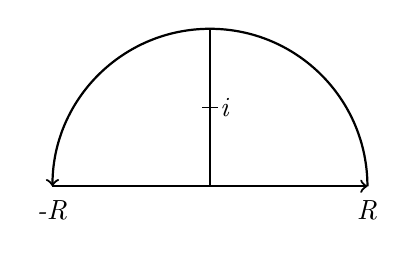
\begin{tikzpicture}
        % Draw horizontal base line
        \draw[->,thick] (-2,0) -- (2,0);
        
        % Draw vertical radius
        \draw[thick] (0,0) -- (0,2);
        
        % Indicate current direction
        \draw[->,thick] (2,0) arc[start angle=0,end angle=180,radius=2cm];
        
        % Small tick mark at center
        \draw (-0.1,1) -- (0.1,1);
        
        % Label current 'i'
        \node at (0.2,1) {\textit{i}};

        % label 'R' and '-R'
        \node at (2,-0.3) {\textit{R}};
        \node at (-2,-0.3) {\textit{-R}};
    \end{tikzpicture}
\end{center}

Since it encloses only $z=i$, if integrate $f(z)$ along the contour of the semicircle, we'll get:
$$\int_{-R}^{R}f(x)dx+\int_{C_R}f(z)dz = 2\pi i\cdot Res_{z=i}f(z)=2\pi i\cdot (-\frac{1}{4}(1-2\pi \zeta)ie^{2\pi \zeta}) = \frac{\pi}{2}(1-2\pi\zeta)e^{2\pi\zeta}$$
Then, using similar technique from previous part, we can prove that $\lim_{R\rightarrow\infty}\int_{C_R}f(z)dz = 0$.

Hence, $\lim_{R\rightarrow\infty}\int_{-R}^{R}f(x)dx = \int_{-\infty}^{\infty}f(x)dx = -2\pi(1-2\pi\zeta)e^{2\pi\zeta}$.

Since $\zeta<0$, then it is then characterized as:
$$\int_{-\infty}^{\infty}f(x)dx =\int_{-\infty}^{\infty}\frac{e^{-2\pi ix\zeta}}{(1+x^2)^2}dx = \frac{\pi}{2}(1+2\pi|\zeta|)e^{-2\pi|\zeta|}$$

So, regardless of the sign of $\zeta$, the following integral is always true:
$$\int_{-\infty}^{\infty}\frac{e^{-2\pi ix\zeta}}{(1+x^2)^2}dx = \frac{\pi}{2}(1+2\pi|\zeta|)e^{-2\pi|\zeta|}$$

\hfil

\hfil

\section*{6}
\begin{myBox}[]{}
    \begin{question}
        Stein and Shakarchi Pg. 104 Problem 10:

        Show that if $a>0$, then
        $$\int_{0}^{\infty}\frac{\log x}{x^2+a^2}dx = \frac{\pi}{2a}\log a$$
    \end{question}
\end{myBox}

\textbf{Pf:}

Choose $0<\epsilon<a$, and $R>a$. Construct the semicircle $C_\epsilon$ and $C_R$ for upper half plane, with $C_r$ being characterized by $z=re^{i\theta}$ with $\theta\in[0,\pi]$.
Along with two straight lines $\gamma$ on real axis parametrized by $\epsilon\leq |x|\leq R$, we can create a contour with the following orientation:

\begin{center}
    \includegraphics*[width = 60mm]{complex problem 6.png}
\end{center}

Before starting, we need to redefine the logarithmic function, so that the region we're integrating over has a single-valued branch.
Define the domain to be $\mathbb{C}\setminus\{ix\ |\ x\leq 0\}$, and for all $z$ in the domain, $\log(z)=\ln|z|+i\arg(z)$, where $\arg(z)\in (-\frac{\pi}{2},\frac{3\pi}{2})$ (so we can cover the whole real axis except for $0$).

Then, for all $x<0$, $\log(x)=\ln|x|+i\arg(x)=\ln|x|+i\pi$.

\hfil

Now, if we consider the integral of $f(z)=\frac{\log(z)}{z^2+a^2}=\frac{\log(z)}{(z-ia)(z+ia)}$, the contour is enclosing the point $ia$. 
Notice that since $\frac{\log(z)}{(z+ia)}$ is analytic at $ia$, then choose a sufficiently small circle $C$ centered at $ia$, the residue at $ia$ is given as:
$$Res_{z=ia}f(z) = \frac{1}{2\pi i}\int_{C}\frac{\log(z)}{(z+ia)}\cdot\frac{1}{(z-ia)}dz = n(C,ia)\cdot \frac{\log(ia)}{(ia+ia)} = \frac{\ln(a)+i\frac{\pi}{2}}{2ia}$$

So, integrating over the contour with the chosen orientation, we get:
$$\int_{\gamma - C_\epsilon + C_R}f(z)dz = \left(\int_{-R}^{-\epsilon}f(x)dx+\int_{\epsilon}^{R}f(x)dx\right) - \int_{C_\epsilon}f(z)dz + \int_{C_R}f(z)dz$$
$$ = 2\pi i\cdot Res_{z=ia}f(z) = 2\pi i\cdot \frac{\ln(a)+i\frac{\pi}{2}}{2ia} = \frac{\pi}{a}\ln(a)+i\frac{\pi^2}{2a}$$

\hfil

\textbf{Integral over $C_R$:}

Given the parametrization $z=Re^{i\theta}$ with $\theta\in [0,\pi]$ for $C_R$, then the integral is given by:
$$\int_{C_R}f(z)dz = \int_{0}^{\pi}\frac{\log(Re^{i\theta})}{(Re^{i\theta})+a^2}\cdot iRe^{i\theta}d\theta = \int_{0}^{\pi}\frac{\ln(R) + i\theta}{(Re^{i\theta})^2+a^2}\cdot iRe^{i\theta}d\theta$$
Since $0\leq \theta \leq \pi$ for variable $\theta$, then the modulus of the integral can be bounded by:
$$\left|\int_{C_R}f(z)dz\right|\leq \int_{0}^{\pi}\frac{|\ln(R) + i\theta|}{|(Re^{i\theta})^2+a^2|}|iRe^{i\theta}|d\theta \leq \int_{0}^{\pi}\frac{\sqrt{(\ln(R))^2+\theta^2}}{|Re^{i\theta}|^2-|a|^2}Rd\theta \leq \int_{0}^{\pi}\frac{\sqrt{(\ln(R))^2+\pi^2}}{R^2-a^2}Rd\theta$$
$$\leq \int_{0}^{\pi}\frac{|\ln(R)|+|\pi|}{R^2-a^2}Rd\theta = \frac{\pi(|\ln(R)|+\pi)}{R^2-a^2}R$$
WLOG, can assume the initial choice of $R\geq 1$, hence $\ln(R)\geq 0$, so $|\ln(R)|=\ln(R)$.

Then, as $R\rightarrow\infty$, we get:
$$0\leq \lim_{R\rightarrow\infty}\left|\int_{C_R}f(z)dz\right| \leq \lim_{R\rightarrow\infty}\frac{\pi(\ln(R)+\pi)R}{R^2-a^2} = \lim_{R\rightarrow\infty}\frac{\pi(\ln(R)+1+\pi)}{2R} = \lim_{R\rightarrow\infty}\frac{\pi/R}{2} = 0$$
(Note: the above limit is given by L'hopital's Rule).

Hence, $\lim_{R\rightarrow\infty}\int_{C_R}f(z)dz = 0$.

\hfil

\textbf{Integral over $C_\epsilon$:}

Given the parametrization $z=\epsilon e^{i\theta}$ with $\theta\in [0,\pi]$ for $C_\epsilon$, then the integral is given by:
$$\int_{C_\epsilon}f(z)dz = \int_{0}^{\pi}\frac{\log(\epsilon e^{i\theta})}{(\epsilon e^{i\theta})^2+a^2}i\epsilon e^{i\theta}d\theta=\int_{0}^{\pi}\frac{\ln(\epsilon)+i\theta}{(\epsilon e^{i\theta})^2+a^2}i\epsilon e^{i\theta}d\theta$$
Based on similar argument, the modulus of the integral can be bounded by:
$$\left|\int_{C_\epsilon}f(z)dz\right|\leq \int_{0}^{\pi}\frac{|\ln(\epsilon)+i\theta|}{|(\epsilon e^{i\theta})^2+a^2|}|i\epsilon e^{i\theta}|d\theta \leq \int_{0}^{\pi}\frac{\sqrt{(\ln(\epsilon))^2+\theta^2}}{||\epsilon e^{i\theta}|^2-a^2|}\epsilon d\theta \leq \int_{0}^{\pi}\frac{|\ln(\epsilon)|+|\theta|}{a^2-\epsilon^2}\epsilon d\theta$$
$$\leq \int_{0}^{\pi}\frac{|\ln(\epsilon)|+|\pi|}{a^2-\epsilon^2}\epsilon d\theta\leq \frac{\pi(|ln(\epsilon)|+\pi)}{a^2-\epsilon^2}\epsilon = \frac{\pi|\ln(\epsilon)|\epsilon +\pi^2\epsilon}{a^2-\epsilon^2}$$
WLOG, can assume $\epsilon<1$, hence $\ln(\epsilon)<0$, or $|\ln(\epsilon)|=-\ln(\epsilon)$ for simplicity.

Then, as $\epsilon\rightarrow 0$, the following limits are true:
$$\lim_{\epsilon\rightarrow 0^+}\frac{1}{a^2-\epsilon^2} = \frac{1}{a^2},\quad \lim_{\epsilon\rightarrow 0^+}\pi^2\epsilon = 0,\quad \lim_{\epsilon\rightarrow 0^+}-\pi\ln(\epsilon)\epsilon = \lim_{\epsilon\rightarrow 0^+}-\pi\frac{\ln(\epsilon)}{1/\epsilon} = \lim_{\epsilon\rightarrow 0^+}-\pi\frac{1/\epsilon}{-1/\epsilon^2} = \lim_{\epsilon\rightarrow 0^+}\pi \epsilon = 0$$
Hence:
$$\lim_{\epsilon\rightarrow 0^+}\frac{\pi|\ln(\epsilon)|\epsilon +\pi^2\epsilon}{a^2-\epsilon^2} = \lim_{\epsilon\rightarrow 0^+}\frac{-\pi\ln(\epsilon)\epsilon +\pi^2\epsilon}{a^2-\epsilon^2} = \frac{0+0}{a^2}=0$$
So, $\lim_{\epsilon\rightarrow 0^+}\int_{C_\epsilon}f(z)dz = 0$.

\hfil

\textbf{Original Integral:}

To retrieve the original integral $\int_{0}^{\infty}\frac{\log(x)}{x^2+a^2}dx$, we need $R\rightarrow\infty$ and $\epsilon\rightarrow 0^+$. So, the following is true:
$$\lim_{R\rightarrow\infty}\lim_{\epsilon\rightarrow 0^+}\left(\int_{-R}^{-\epsilon}f(x)dx+\int_{\epsilon}^{R}f(x)dx\right) - \int_{C_\epsilon}f(z)dz + \int_{C_R}f(z)dz$$
$$ = \int_{-\infty}^{0^-}f(x)dx + \int_{0^+}^{\infty}f(x)dx - \lim_{\epsilon\rightarrow 0^+}\int_{C_\epsilon}f(z)dz + \lim_{R\rightarrow\infty}\int_{C_R}f(z)dz$$
$$ = \int_{-\infty}^{0^-}f(x)dx + \int_{0^+}^{\infty}f(x)dx$$

Input the function $f(z)$, we get:
$$\int_{-\infty}^{0^-}f(x)dx + \int_{0^+}^{\infty}f(x)dx = \int_{-\infty}^{0^-}\frac{\log(x)}{x^2+a^2}dx + \int_{0^+}^{\infty}\frac{\log(x)}{x^2+a^2}dx$$
$$=\int_{-\infty}^{0^-}\frac{\ln|x|+i\pi}{x^2+a^2}dx + \int_{0^+}^{\infty}\frac{\ln|x|}{x^2+a^2}dx = \left(\int_{-\infty}^{0^-}\frac{\ln|x|}{x^2+a^2}dx + \int_{0^+}^{\infty}\frac{\ln|x|}{x^2+a^2}dx\right)+i\int_{-\infty}^{0^-}\frac{\pi}{x^2+a^2}dx$$
Also, recall that the above quantity equals to $\frac{\pi}{a}\ln(a)+i\frac{\pi^2}{2a}$ by Residue Formula. Then:
$$\left(\int_{-\infty}^{0^-}\frac{\ln|x|}{x^2+a^2}dx + \int_{0^+}^{\infty}\frac{\ln|x|}{x^2+a^2}dx\right) = Re\left(\frac{\pi}{a}\ln(a)+i\frac{\pi^2}{2a}\right) = \frac{\pi}{a}\ln(a)$$
Lastly, since the function $\frac{ln|x|}{x^2+a^2}$ is in fact an even function, then $\int_{0^+}^{\infty}\frac{\ln|x|}{x^2+a^2}dx$ is half of the above quantity, or $\frac{\pi}{2a}\ln(a)$.
Hence:
$$\int_{0}^{\infty}\frac{\ln(x)}{x^2+a^2}dx = \frac{\pi}{2a}\ln(a)$$

\break

\section*{7}
\begin{myBox}[]{}
    \begin{question} Stein and Shakarchi Pg. 104 Problem 11
        :

        Show that if $|a|<1$, then
        $$\int_{0}^{2\pi}\log|1-ae^{i\theta}|d\theta =0$$
        Then, prove that the above result remains true if we assume only that $|a|\leq 1$.
    \end{question}
\end{myBox}

\textbf{Pf:}

\textbf{When $|a|<1$:}

If $a=0$, the case is trivial (since $\log|1-ae^{i\theta}| = \log|1|=0$, then the whole integral is $0$). So, assume $a\neq 0$.

\hfil

Consider the integral of $\log(1-z)/iz$ along a circle $C$ of radius $|a|<1$ centered at $0$. With the parametrization $z=ae^{i\theta}$ ($\theta\in [0,2\pi]$), it can be expressed as:
$$I=\int_{C}\frac{\log(1-z)}{iz}dz = \int_{0}^{2\pi}\frac{\log(1-ae^{i\theta})}{iae^{i\theta}}(iae^{i\theta})d\theta = \int_{0}^{2\pi}\log(1-ae^{i\theta})d\theta$$
Which, define the domain to be $\mathbb{C}\setminus\{x\geq 1\}$, and $\log(1-z)=\ln|1-z|+i\arg(1-z)$, it can also be expressed as:
$$I= \int_{0}^{2\pi}\log(1-ae^{i\theta})d\theta=\int_{0}^{2\pi}\ln|1-ae^{i\theta}|d\theta + i\int_{0}^{2\pi}\arg(1-ae^{i\theta})d\theta$$

Going back to the original integral, since the function $-\frac{\log(1-z)}{i}$ is analytic on the domain $\mathbb{C}\setminus\{x\geq 1\}$, so on the disk enclosed by $C$, the only Pole 
is generated by $\frac{1}{z}$ (at the origin). Hence, let $\phi(z)=\frac{\log(1-z)}{i}$, the integral is then characterized by Cauchy's Integral Formula:
$$\int_{C}\frac{\log(1-z)}{iz}dz = \int_{C}\frac{\phi(z)}{z}dz = 2\pi i\cdot n(C,0)\phi(0)$$
With $n(C,0)=1$ (winding number $1$ by our construction), and $\phi(0)=\log(1-0)/(i\cdot 1)=0$, then such integral is evaluated to be $0$.

Now, since $Re(I) = \int_{0}^{2\pi}\log|1-ae^{i\theta}|d\theta$, while $I=0$, then this integral must also evaluated to be $0$.

\hfil

\textbf{Case when $|a|=1$ (Real Integral Approach):}

For $|a|=1$, WLOG, we can assume $a=1$ (since other than that, any $e^{i\phi}$ is adding a phase of $\phi$, which by changing the range of our integrand, we can modify it to be the same as $a=1$).

Then, the integral can be rewrite as:
$$\int_{0}^{2\pi}\ln|1-e^{i\theta}|d\theta = \int_{0}^{2\pi}\ln|1-(\cos(\theta)+i\sin(\theta))|d\theta = \int_{0}^{2\pi}\ln\sqrt{(1-\cos(\theta))^2+(-\sin(\theta))^2}d\theta$$
$$=\int_{0}^{2\pi}\ln\sqrt{1+\cos^2(\theta)-2\cos(\theta)+\sin^2(\theta)}d\theta = \int_{0}^{2\pi}\ln\left((2-2\cos(\theta))^\frac{1}{2}\right)d\theta$$
$$=\frac{1}{2}\int_{0}^{2\pi}\ln\left(4\left(\frac{1-\cos(\theta)}{2}\right)\right)d\theta = \frac{1}{2}\int_{0}^{2\pi}\ln\left(2^2\cdot \sin^2\left(\frac{\theta}{2}\right)\right)d\theta$$
$$ = \frac{1}{2}\cdot 2\int_{0}^{2\pi}\ln\left(2\sin\left(\frac{\theta}{2}\right)\right)d\theta$$
Using the substitution $u=\frac{\theta}{2}$ (with $2du = d\theta$), it can be modified to:
$$\frac{1}{2}\cdot 2\int_{0}^{2\pi}\ln\left(2\sin\left(\frac{\theta}{2}\right)\right)d\theta = 2\int_{0}^{\pi}\ln(2\sin(u))du = 2\int_{0}^{\pi}(\ln(2)+\ln(\sin(u)))du$$
$$ = 2\pi\ln(2) + 2\int_{0}^{\pi}\ln(\sin(u))du$$

So, it suffices to show the integral of $\ln(\sin(u))$ from $0$ to $\pi$.

\hfil

Notice that since $\sin(u)=\sin(\pi-u)$, then for the following integral, do the substitution $\theta=\pi-u$ (or $-d\theta = du$), we can do the following:
$$\int_{\frac{\pi}{2}}^{\pi}\ln(\sin(u))du = \int_{\frac{\pi}{2}}^{\pi}\ln(\sin(\pi-u))du = -\int_{\frac{\pi}{2}}^{0}\ln(\sin(\theta))d\theta = \int_{0}^{\frac{\pi}{2}}\ln(\sin(\theta))d\theta$$
So, the following is true:
$$\int_{0}^{\pi}\ln(\sin(u))du = 2\int_{0}^{\frac{\pi}{2}}\ln(\sin(u))du$$
Let $I=\int_{0}^{\frac{\pi}{2}}\ln(\sin(u))du$, using the fact that $\sin(u)=\cos(\frac{\pi}{2}-u)$, with substitution $\theta=\frac{\pi}{2}-u$ (or $-d\theta=du$), we can again get:
$$I=\int_{0}^{\frac{\pi}{2}}\ln\left(\cos\left(\frac{\pi}{2}-u\right)\right)du = -\int_{\frac{\pi}{2}}^{0}\ln(\cos(\theta))d\theta = \int_{0}^{\frac{\pi}{2}}\ln(\cos(\theta))d\theta$$
So, we can also get the following:
$$2I=\int_{0}^{\frac{\pi}{2}}\ln(\sin(u))du+\int_{0}^{\frac{\pi}{2}}\ln(\cos(u))du = \int_{0}^{\frac{\pi}{2}}\ln(\sin(u)\cos(u))du = \int_{0}^{\frac{\pi}{2}}\ln\left(\frac{1}{2}\sin(2u)\right)du$$
$$=\int_{0}^{\frac{\pi}{2}}\left(\ln\left(\frac{1}{2}\right)+\ln(\sin(2u))\right)du = -\frac{\pi}{2}\ln(2) + \int_{0}^{\frac{\pi}{2}}\ln(\sin(2u))du$$
Using the substitution $\theta=2u$ (with $\frac{1}{2}d\theta=du$), we get the following:
$$2I = -\frac{\pi}{2}\ln(2)+\frac{1}{2}\int_{0}^{\pi}\ln(\sin(\theta))d\theta$$
But, recall the fact that $\int_{0}^{\pi}\ln(\sin(u))du = 2\int_{0}^{\frac{\pi}{2}}\ln(\sin(u))du = 2I$. So, we gt:
$$2I=-\frac{\pi}{2}\ln(2)+\frac{1}{2}\cdot 2I = -\frac{\pi}{2}\ln(2)+I,\quad I=-\frac{\pi}{2}\ln(2)$$

Substituting back to the original integral, we get the following:
$$\int_{0}^{\pi}\ln(\sin(u))du = 2I = -\pi\ln(2)$$
Finally, we get that the original integral is given by:
$$\int_{0}^{2\pi}\ln|1-e^{i\theta}|d\theta = 2\pi\ln(2) + 2\int_{0}^{\pi}\ln(\sin(u))du = 2\pi\ln(2)+2(-\pi\ln(2))=0$$
Hence, we can say it is possible to extend to the case $|a|=1$, so the integral is true for all $|a|\leq 1$.



\end{document}